
\marginpar{\href{https://youtu.be/-qCEoqpwjf4}{Video}} Reading: 2.4-2.6

RV is a function from the sample space to the real numbers: $\Omega \rightarrow \mathbb{R}$

\marginpar{(8m)}

\begin{align*}
E[X-E[X]] = E[X] - E[X] = 0
\end{align*}

If we want to say something about how far we are from the mean, could take $|abs|$.

\begin{align}
var(X)=E[(X-E[X])^2] = \sum_x(x - E[X])^2 p_X(x)\\
= E[X^2] -(E[X])^2
\end{align}
\myequations{Definition of Variance}

std = $\sigma_X = \sqrt{var(X)}$

\subsection{Random Speed}

\marginpar{(12m)}

Traverse 200 mile distance at constant but random speed v.


\begin{figure}[h]
\begin{tikzpicture}
\centering
\begin{axis}[
    % axis lines = left,
   xtick={1,200},
    ytick={.5,.5},
]
\addplot+[ycomb] plot coordinates
    {(1,.5) (200,.5) };
\end{axis}
\end{tikzpicture}
\caption{$p_V(v)$}
\end{figure}

$d=200$, $T=t(v)-200/v$

\begin{align*}
E[V] = \frac{1}{2}1 + \frac{1}{2}200 = 100.5
\end{align*}

\begin{align*}
var[V] = \frac{1}{2}(1-100.5)^2 + \frac{1}{2}(200 -100.5)^2 = 100^2
\end{align*}

$\sigma_V = \sqrt{100^2}=100$

\marginpar{(14:15)}

Random variable T: time in hours=T=$T(v)=$

\begin{align*}
E[T] = E[t(v)] = \sum_v t(v)p_V(v) = \frac{1}{2}200 + \frac{1}{2}2 = 100.5
\end{align*}

\begin{align*}
E[TV] = 200 \ne E[T]E[V]
\end{align*}

\begin{align*}
E[200/V] = E[T] \ne 200/E[V] \approx 2
\end{align*}

\subsection{Conditional PMF and Expectation}

\marginpar{(18m)}

\begin{align*}
p_{X|A}(x) = P(X=x|A)\\
E[X|A] = \sum_x x p_{X|A}(A) ???check
\end{align*}

Let $A=(X \ge 2)$

\begin{align*}
p_{X|A}(x) = \frac{1}{3},\; x=2,3,4
\end{align*}

Conditional PMF's need to add to 1.

\begin{align*}
E[X|A] = \frac{1}{3}2 + \frac{1}{3}3 + \frac{1}{3}4=3
\end{align*}


\begin{figure}[h]
\centering
\begin{tikzpicture}
\begin{axis}[
    % axis lines = left,
   xtick={1,2,3,4},
    ytick={0,.25,1},
]
\addplot+[ycomb] plot coordinates
    % {(0,.25) (1,.25) (2,.25) (3,.25) (4,.25)};
    {(1,.25) (2,.25) (3,.25) (4,.25)};
\end{axis}
\end{tikzpicture}
\caption{$p_X(x)$}
\end{figure}

\marginpar{(23:25)}

\subsection{Geometric PMF}
\marginpar{(24:50)}

\subsection{Total Expectation Theorem}

\marginpar{(34:30)}

Partition sample space into disjoint events $A_1, \ldots, A_n$

Divide and Conquer method.

\begin{figure}[h]
\centering
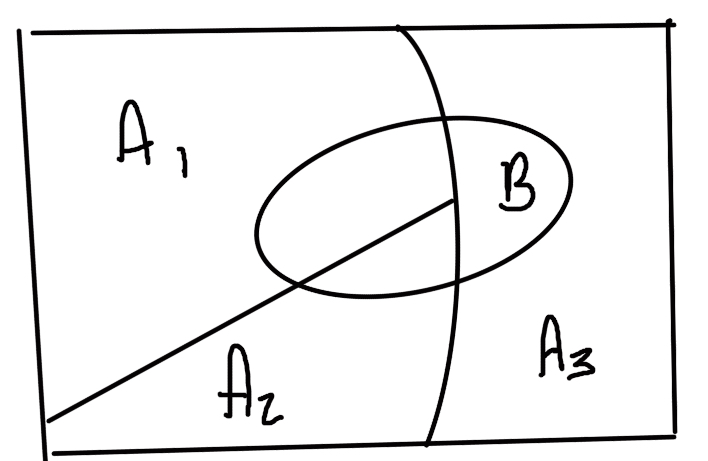
\includegraphics[width=5cm, height=4cm]{images/L02/total_prob.jpeg}
\caption{Total Probability}
\end{figure}

\begin{align}
P(B)=P(A_1)P(B|A_1) + \cdots + P(A_n)P(B|A_n) - \text{Total Probability Theorem} \\
?? p_X(x) = P(A_1)p_{X|A_1}(x) + \cdots + P(A_n)p_{X|A_n}(x) - \text{Translated with PMF's}
\end{align}
\myequations{Total Probability Theorem}

\begin{align*}
E[X]=P(A_1)E(X \mid A_1) + \cdots + P(A_n)E(X \mid A_n)
\end{align*}

\subsection{Divide and Conquer with Geometric Variable}

\marginpar{(37:25)}

$A_1:\{X=1\}, A_2:\{X >1\}$

\begin{align*}
E[X]=P(X=1)E(X|X=1) + P(X > 1)E(X \mid X>1)
\end{align*}
Solve to get $E[X]=\frac{1}{p}$

\begin{align*}
E[X|X-1 >0] = E[X-1 \mid X-1>0] + 1 ??
\end{align*}

\subsection{Joint PMFs}

\marginpar{(48:30)} Joint probabilities

\begin{figure}[h]
\centering
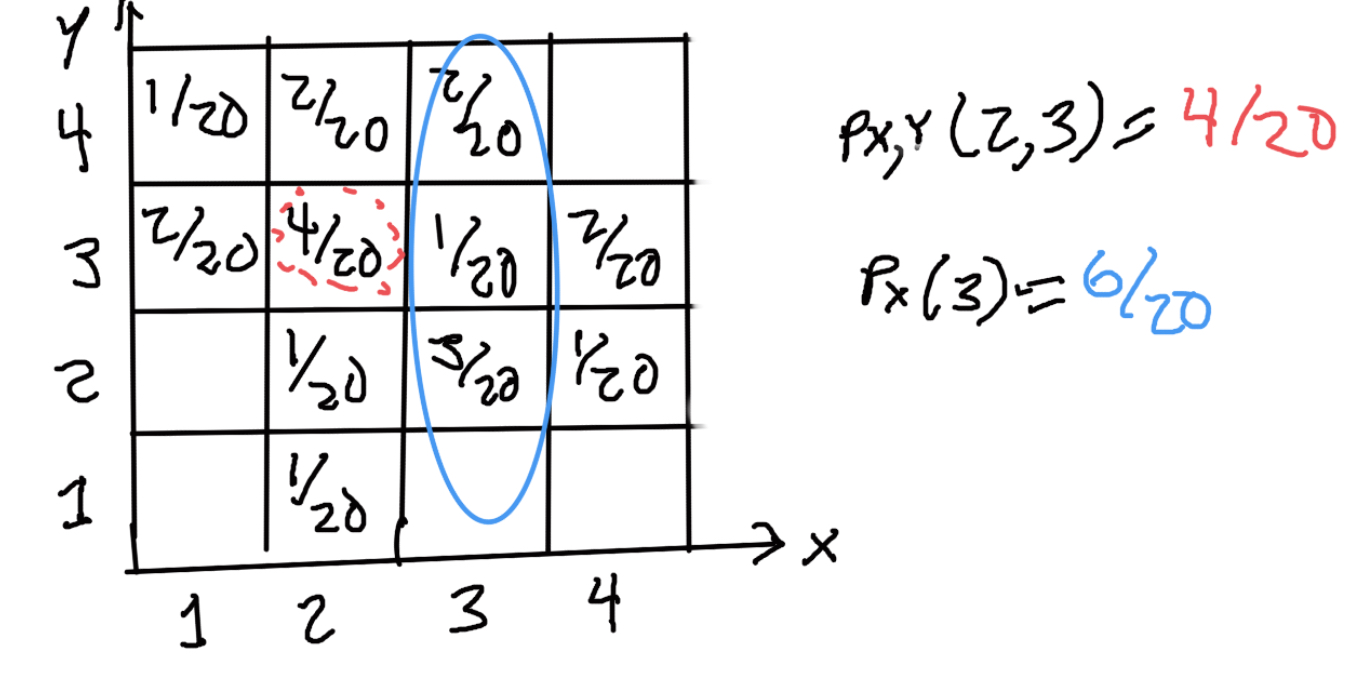
\includegraphics[width=8cm, height=4cm]{images/L06/joint_pmf.jpeg}
\caption{Joint PMFs}
\end{figure}
